\section{Kakas Pengembangan}

Pada tugas akhir ini terdapat beberapa kakas yang digunakan untuk memanfaatkan metode PEFT pada tugas evaluasi IndoLEM, kakas tersebut yaitu Transformers dari Huggingface dan Adapters. Pada subbab ini dijelaskan mengenai masing-masing kakas tersebut.

\subsection{Transformers}

Transformers merupakan pustaka kolektif (\textit{open-source}) yang diinisialisasi oleh Huggingface. Transformers berfungsi sebagai pustaka yang dapat diakses secara umum terkait dengan arsitektur Transformer \parencite{huggingface}. Pustaka ini berisi berbagai macam \textit{pre-trained model} berbasis arsitektur Transformer yang dapat digunakan melalui pustaka tersebut, sehingga memudahkan pengguna untuk memakai model \parencite{huggingface}.

\begin{figure}[h]
    \vspace{0.25cm}
    \centering
    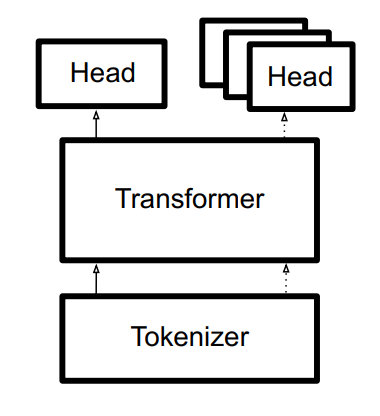
\includegraphics[width=0.6\textwidth]{chapter-2/huggingface.png}
    \caption{Komponen dari Model pada Transformers \parencite{huggingface}}
    \label{fig:huggingface}
\end{figure}

Setiap model pada pustaka Transformers terdiri dari tiga komponen yaitu, Tokenizer, Transformer, dan Head, seperti yang bisa dilihat pada gambar \ref{fig:huggingface} \parencite{huggingface}. Komponnen Tokenizer berfungsi untuk melakukan tokenisasi atau melakukan konversi dari teks asli ke sebuah \textit{enconding} \parencite{huggingface}. Lalu, komponen Transformer melanjutkan hasil dari Tokenizer tersebut, yaitu mengubah \textit{encoding} menjadi \textit{contextual embedding} \parencite{huggingface}. Terakhir, komponen Head akan mengubah \textit{contextual embedding} dari komponen Transformer menjadi sebuah prediksi yang spesifik kepada tugas evaluasi yang sedang dilatih \parencite{huggingface}.

\begin{table}[h]
    \caption{Contoh kode penggunaan Transformers}
    \label{table:huggingface-model-code}
    \begin{lstlisting}[language=python]
    tknzr = AutoTokenizer.from_pretrained("bert-base-uncased")
    model = AutoModel.from_pretrained("bert-base-uncased")
    \end{lstlisting}
\end{table}

Tabel \ref{table:huggingface-model-code} adalah contoh pemanggilan model dengan menggunakan Transformers. \texttt{AutoTokenizer} merupakan komponen Tokenizer yang berfungsi sebagai tokenisasi dan \texttt{AutoModel} merupakan komponen Transformer sebagai \textit{pre-trained model} yang digunakan. Komponen Head dapat ditambahkan dengan menambahkan tugas evaluasi spesifik di belakang pemanggilan model, sebagai contoh untuk tugas klasifikasi akan ditambahkan \texttt{ForSequenceClassification} pada model, sehingga menjadi \texttt{AutoModelForSequenceClassification}.

\begin{table}[h]
    \caption{Argumen pada modul Trainer}
    \label{table:huggingface-trainer-code}
    \begin{lstlisting}[language=python]
    (
        model: Union = None,
        args: TrainingArguments = None,
        data_collator: Optional = None,
        train_dataset: Union = None,
        eval_dataset: Union = None,
        tokenizer: Optional = None,
        model_init: Optional = None,
        compute_metrics: Optional = None,
        callbacks: Optional = None,
        optimizers: Tuple = (None, None),
        preprocess_logits_for_metrics: Optional = None
    )
    \end{lstlisting}
\end{table}

Pustaka Transformers juga menyediakan modul Trainer yang berfungsi untuk pelatihan model. Pelatihan ini dilakukan dengan menggunakan pustaka PyTorch, sehingga mampu menggunakan CUDA yang berfungsi untuk melatih model secara paralel. Argumen yang digunakan pada modul Trainer dapat dilihat pada tabel \ref{table:huggingface-trainer-code}. \textit{Hyperparameter} untuk pelatihan dapat diatur dari model \texttt{TrainingArguments}.

Modul lain yang umum digunakan adalah HfArgumentParser yang berfungsi untuk melakukan \textit{parsing} terhadap argumen yang digunakan. Modul ini akan membaca argumen yang diberikan oleh pengguna melalui \textit{script}, lalu hasil pembacaan tersebut dapat digunakan. Argumen yang diterima bukan hanya argumen untuk pelatihan (\textit{hyperparameter}), dapat dibuat kelas untuk melakukan \textit{parsing} terhadap argumen lain, salah satunya adalah untuk \textit{dataset}. Untuk dokumentasi yang lengkap terkait pustaka Transformers dapat dilihat pada tautan berikut \url{https://huggingface.co/docs/transformers}.

\subsection{Adapters}

Adapters merupakan pustaka kolektif (\textit{open-source}) yang diinisialisasi oleh \citeauthor{adapters}. Pustaka Adapters merupakan penyatuan dari berbagai metode PEFT \parencite{adapters}. Terdapat beberapa metode PEFT yang diimplementasikan pada pustaka tersebut salah satunya adalah \textit{Adapter}, \textit{Prefix-Tuning}, LoRA, IA3, dan lain-lain. Metode PEFT yang tersedia beserta konfigurasi penggunaannya dapat dilihat pada tabel \ref{table:adapters-method}. 

\begin{table}[h]
    \vspace{0.25cm}
    \centering
    \caption{Metode PEFT pada pustaka Adapters dan konfigurasinya \parencite{adapters}}
    \label{table:adapters-method}
    \begin{tabular}{ll}
        \toprule
        \textbf{Method Name} & \textbf{Default Config} \\
        \midrule
        Bottleneck adapter \parencite{adapter_houlsby} & \texttt{[double\_]seq\_bn} \\
        Invertible adapter \parencite{adapter_pfeiffer} & \texttt{seq\_bn\_inv} \\
        Prompt tuning \parencite{prompt_tuning} & \texttt{prompt\_tuning} \\
        Prefix tuning \parencite{prefix_tuning} & \texttt{prefix\_tuning} \\
        Compacter \parencite{compacter} & \texttt{compacter} \\
        LoRA \parencite{lora} & \texttt{lora} \\
        (IA)$^3$ \parencite{ia3} & \texttt{ia3} \\
        Parallel adapter \parencite{uvpl} & \texttt{par\_bn} \\
        Mix-and-Match adapter \parencite{uvpl} & \texttt{mam} \\
        UniPELT \parencite{unipelt} & \texttt{unipelt} \\
        \bottomrule
    \end{tabular}
\end{table}

Adapters merupakan penelitian selanjutnya dari AdapterHub yang merupakan \textit{fork} dari pustaka Transformers \parencite{adapters}. Sehingga, implementasinya didasarkan pada kode yang termuat pada pustaka Transformers. Pustaka Adapters menawarkan integrasi dengan pustaka Transformers, \textit{script} adaptasi untuk penggunaan metode PEFT, dan juga fungsionalitas untuk menyimpan dan memuat metode PEFT yang telah dilatih \parencite{adapters}.

\begin{table}[h]
    \caption{Contoh kode penggunaan Adapters}
    \label{table:adapters-code}
    \begin{lstlisting}[language=python]
    import adapters
    from transformers import AutoModel
    model = AutoModel.from_pretrained("..")
    adapters.init(model)
    model.add_adapter("a", config="seq_bn")
    model.add_adapter("b", config="seq_bn")
    model.train_adapter(Parallel("a", "b"))
    \end{lstlisting}
\end{table}

Tabel \ref{table:adapters-code} menunjukkan contoh kode untuk penggunaan metode PEFT pada pustaka Adapters. Metode PEFT diinisialisasi dengan menggunakan fungsi \texttt{init}, lalu ditambahkan dengan \texttt{add\_adapter}. Untuk melatih metode PEFT, sehingga hanya melatih parameter dari metode PEFT tersebut (\textit{freeze} pada parameter asli model), perlu dilakukan pemanggilan pada fungsi \texttt{train\_adapter}. Model tidak harus diinisialisasi dengan menggunakan fungsi \texttt{init}, melainkan dapat diinisialisasi dengan memanggil \texttt{XXXAdapterModel} yang mirip dengan penggunaan pada Transformers. Sebagai contoh, \texttt{XXXAdapterModel} dapat digunakan dengan memanggil \texttt{AutoAdapterModel}. Modul Trainer juga terdapat ekuivalen untuk PEFT-nya yaitu AdapterTrainer. Begitu pula dengan TrainingArgument, terdapat AdapterArguments sebagai \textit{hyperparameter} dari metode PEFT. Untuk dokumentasi yang lengkap terkait pustaka Adapters dapat dilihat pada tautan berikut \url{https://docs.adapterhub.ml/}.
